\documentclass[11pt]{article}

\usepackage[T1]{fontenc}
\usepackage[french]{babel}
\usepackage[utf8]{inputenc}

\newcommand{\mg}{25mm}
\usepackage[left=\mg,right=\mg,top=\mg,bottom=\mg]{geometry}

\usepackage{graphicx}
\usepackage{color}
\definecolor{navy}{RGB}{32,11,140}

\linespread{1.3}

\usepackage[colorlinks=true,linkcolor=navy]{hyperref}

\begin{document}

  \sffamily

  \begin{center}
    \bfseries
      \Huge{MazeML}\\
      \Large{Concours du Site du Zéro}\\
      \rule{0.8\linewidth}{5\em}
    \vspace*{20\em}
  \end{center}

  \tableofcontents
  \pagebreak

  C'est les vacances, autant en profiter. Comme ce concours n'est pas noté, et 
  qu'il propose un sujet intéressant, il est assez tentant de s'y pencher\ldots\
  d'ailleurs c'est ce que j'ai fait.

  \vspace{3mm}

  En plus, il y a généralement peu de codes écrits en OCaml\ldots\ donc cette 
  contribution pourra servir d'exemple à ceux qui veulent s'y mettre. Elle 
  permet d'ailleurs d'illustrer l'utilisation de LablGTK, ainsi que d'autres 
  choses plus ou moins importantes :

  \vspace{3mm}
  \begin{itemize}
    \item Découpage du code en modules;
    \item Dessin et double buffering;
    \item Et bien sûr la partie algorithmique elle-même !
  \end{itemize}
  \vspace{3mm}

  Bon, assez de paroles ! Venons-en aux faits.


  \section{Introduction}

  J'ai choisi de n'implémenter qu'une partie des fonctionnalités présentées sur
  la page principale du concours et, en toute franchise, je n'ai pas l'intention
  d'en faire plus (c'est pour moi un « projet-jouet » pour m'amuser, auquel je 
  ne peux pas consacrer \emph{tout} le temps que je voudrais). Concrètement, 
  voici ce que fait ce programme :

  \vspace{3mm}
  \begin{itemize}
    \item Créer des labyrinthes parfaits de 4 $\times$ 4 à 240 $\times$ 390 
      cases.
    \item Afficher la solution des labyrinthes créés.
    \item Construire pas à pas un labyrinthe.
    \item Enregistrer et charger des labyrinthes.
    \item Exporter des labyrinthes sous forme d'image (PNG, JPEG ou BMP).
  \end{itemize}


  \section{Caractéristiques du programme}

    \subsection{Nom}

    Ce programme s'appelle MazeML, nom composé du mot anglais \textit{maze}, qui
  signifie labyrinthe, et du suffixe ML, pour rappeler qu'il a été écrit en 
  OCaml.

    \subsection{Licence}

    MazeML est distribué sous les termes de la licence GNU GPL version 3. Une 
  copie est incluse dans l'archive contenant les sources.

    \subsection{Labyrinthes}

    MazeML permet de dessiner des labyrinthes de $4 \times 4$ à $240 \times 390$
  cases. Ces limites sont imposées par la taille réduite de la zone de dessin 
  (fixe\ldots on peut envisager de la rendre redimensionnable, et permettre 
  ainsi de tracer de plus gros labyrinthes, mais je ne le ferai pas).

  \vspace{3mm}
  \textbf{Remarque} : depuis la version 1.8, l'option \texttt{--without-gui} 
  permet de créer et d'exporter de gros labyrinthes (testé jusqu'à 
  $700 \times 700$ cases) au format PNG. Il s'agit surtout d'une fonctionnalité
  \emph{pour le fun} car l'export au format PNG est très lent et 
  \texttt{GtkDrawable} n'est pas l'outil le plus approprié pour des dessins de 
  cette envergure. De toutes façons, le programme échoue dès $800 \times 800$ 
  avec un bel \texttt{Out of memory}.

    \subsection{Algorithme}

    MazeML crée des labyrinthes grâce à l'algorithme d'exploration exhaustive. 
  Les informations de backtracking sont stockées au fur et à mesure de la 
  progression. Il est alors possible d'écrire une fonction récursive terminale, 
  ce qui évite les débordements de pile pour de gros labyrinthes.

  \vspace{3mm}
  \textbf{Remarque} : Il existe bien entendu de nombreux autres algorithmes plus
  ou moins efficaces pour créer des labyrinthes (avec un biais plus ou moins 
  prononcé). Il est sans doute intéressant d'en implémenter plusieurs et de les 
  comparer, mais je ne le ferai pas.

    \subsection{Résolution du labyrinthe}

    L'algorithme d'exploration exhaustive crée des labyrinthes parfaits. Il 
  n'existe donc qu'un seul chemin pour aller de la case de départ à la case 
  d'arrivée (où qu'elles soient placées). Par conséquent, on peut exploiter 
  astucieusement les données de backtracking pour calculer la solution en même 
  temps que la création du labyrinthe, sans utiliser d'algorithme dédié.

    \subsection{Affichage des labyrinthes}

    MazeML affiche les labyrinthes avec les outils de base que sont 
  \texttt{GtkDrawable} et \texttt{GtkPixmap} (pas d'OpenGL ou de bibliothèque 
  spécialisée). Il s'agit d'une certaine façon d'utiliser des fonctions 
  comparables à celles du module \texttt{Graphics} de la bibliothèque standard 
  d'OCaml. Voici un exemple de tracé :

  \begin{figure}[!ht]
    \centering
    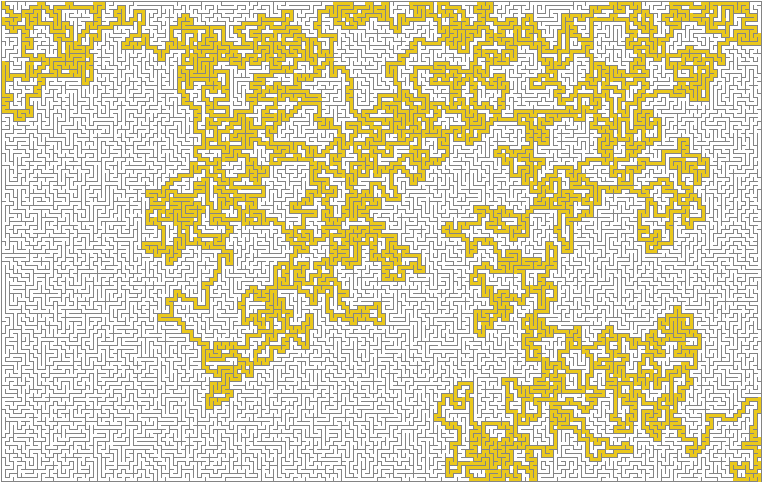
\includegraphics[scale=0.5]{MazeML-somewhat-big-maze.png}
  \end{figure}

    \subsection{Implémentation}

    Les labyrinthes sont représentés par des tableaux de type \texttt{Bigarray} 
  à une dimension, composés d'entiers non signés codés sur 8 bits. Chaque case 
  du labyrinthe est ainsi codée par un octet. Plus précisément :

  \vspace{3mm}
  \begin{itemize}
    \item Les 4 bits de poids fort représentent les portes N (nord), W (ouest), 
    E (est) et S (sud). Ils stockent les informations de backtracking, 
    c'est-à-dire la porte à franchir pour revenir en arrière.
    \item Les 4 bits de poids faible représentent aussi les portes N, W, E et S.
    Ils représentent les portes ouvertes d'une case donnée.
  \end{itemize}
  \vspace{3mm}

  \textbf{Remarque} : Les données de backtracking sont effacées dès qu'elles ont
  été utilisées, sauf si elles font partie du chemin qui relie la case de départ
  (arbitrairement placée en haut à gauche) à la case d'arrivée (arbitrairement
  placée en bas à droite).

    \subsection{Découpage en modules}

    MazeML est organisé en plusieurs modules relativement indépendants les uns 
  des autres. Ce sont :

  \begin{table}[!ht]
    \centering
    \begin{tabular}{cc}
      \textbf{Nom du module} & \textbf{Contenu}                       \\\hline
      \texttt{UI}            & Widgets de l'interface                 \\
      \texttt{Maze}          & Algorithme d'exploration exhaustive    \\
      \texttt{Drawing}       & Tracés et fonctions d'export           \\
      \texttt{Dialog}        & Dialogue avec l'utilisateur            \\
      \texttt{MazeML}        & Callback et point d'entrée
    \end{tabular}
  \end{table}


    \section{Benchmark}

    L'implémentation proposée ici a été testée, \emph{sans affichage}, bien 
  au-delà des limites de MazeML, sur des labyrinthes jusqu'à 15000 cases de 
  côté. Comme il est souvent délicat de tirer une information fiable d'un 
  benchmark, je donne les temps de calcul moyens (10 mesures par taille de 
  labyrinthe) obtenus sur deux machines très différentes (un PC portable assez 
  ancien et un PC de bureau récent) pour 11 tailles de labyrinthes.

  \begin{table}[!ht]
    \centering\sffamily
    \begin{tabular}{|c|c|c|c|}
                                                                          \hline
      \textbf{Taille} & \textbf{Nombre de cases} & \textbf{Test A} (s) 
      & \textbf{Test B} (s)                                             \\\hline
      1000 $\times$ 1000        & $1.0 \cdot 10^6$  & 0.5    &	0.1     \\\hline
      2000 $\times$ 2000        & $4.0 \cdot 10^6$  & 1.8    &	0.5     \\\hline
      3000 $\times$ 3000        & $9.0 \cdot 10^6$  & 4.0    &	1.2     \\\hline
      4000 $\times$ 4000        & $1.6\cdot 10^7$   & 7.1    &	2.2     \\\hline
      5000 $\times$ 5000        & $2.5\cdot 10^7$   & 11     &	3.5     \\\hline
      6000 $\times$ 6000        & $3.6\cdot 10^7$   & 16     &	5.0     \\\hline
      7000 $\times$ 7000        & $4.9\cdot 10^7$   & 21.8   &	6.8     \\\hline
      8000 $\times$ 8000        & $6.4\cdot 10^7$   & 28.3   & 8.9      \\\hline
      9000 $\times$ 9000        & $8.1\cdot 10^7$   & 37     & 11.4     \\\hline
      10\,000 $\times$ 10\,000  & $1.0 \cdot 10^8$  & 48.5   &	14      \\\hline
      15\,000 $\times$ 15\,000  & $2.25\cdot 10^8$  & 	107  &	31.5    \\\hline
    \end{tabular}\\
    \vspace{3mm}\centering\small
    \textbf{(A)} : Acer Aspire 2012 1.5 GHz ;
    \textbf{(B)} : Dell Inspiron 530 (Core 2 Duo 2.83 GHz)
  \end{table}

    Pour reproduire ces résultats sur votre machine, il suffit de compiler 
  séparément le module \texttt{Maze}. Pour cela, ajoutez le point d'entrée 
  suivant dans \texttt{maze.ml} :

\begin{verbatim}
let _ =
  let t0 = Unix.gettimeofday () in
  let maze = make ~rows:1000 ~cols:1000 in
  let t1 = Unix.gettimeofday () in
  Printf.printf "ROWS %d COLS %d MAZE %g TIME %.3f s\n%!"
    maze.rows maze.cols (float maze.last +. 1.0) (t1 -. t0)
\end{verbatim}

puis compilez et exécutez en utilisant la commande suivante :

\begin{verbatim}
  $ ocamlopt -nodynlink -inline 1000000 bigarray.cmxa maze.ml -o maze
  $ ./maze
\end{verbatim}


    \section{Manipulation en ligne de commande}

    MazeML est en partie configurable en ligne de commande (vous pouvez obtenir
  la liste complète des options reconnues grâce à \texttt{-help}). Voici les 
  principales options reconnues :

  \vspace{3mm}
  \begin{description}
    \item[\texttt{-rows}] $n$ : Nombre de lignes.
    \item[\texttt{-cols}] $n$ : Nombre de colonnes.
    \item[\texttt{-wall}] \texttt{#RRGGBB} : Couleur des murs du labyrinthe.
    \item[\texttt{-cell}] \texttt{#RRGGBB} : Couleur des cases de la solution.
  \end{description}


    \section{Édition de labyrinthes}

    C'est un point qui m'intéresse parce qu'il permet d'illustrer l'efficacité 
  des fonctions de type \texttt{map\_file}. MazeML les exploite 
  bien entendu. Il enregistre et charge des labyrinthes stockés dans un simple 
  fichier texte (jeu de caractères ISO-8859-15). Celui-ci se présente sous la 
  forme :

\begin{verbatim}
ROWS 0000 COLS 0000\n
(contenu du tableau)
(contenu du tableau)
(contenu du tableau)
...
(contenu du tableau)
\end{verbatim}

    De façon très générale, pour un labyrinthe de $n$ lignes et $c$ colonnes, la
  taille du fichier est de $n\times c + 20$ octets (ces 20 octets servent pour 
  \texttt{ROWS} et \texttt{COLS} comme indiqué plus haut).


    \section{Export}

    MazeML propose d'exporter les labyrinthes au format PNG (avec transparence)
  ou JPEG. L'export s'effectue avec ou sans la solution du labyrinthe, selon ce
  qui est affiché à l'écran. La couleur rendue transparente peut être modifiée 
  en ligne de commande.


    \section{Construction pas à pas}

    La version 1.7 de MazeML introduit une nouvelle fonctionnalité : la 
  construction pas à pas des labyrinthes. Pour tester cette fonction, vous devez
  lancer le logiciel avec l'option \texttt{-interactive}. Vous pouvez régler la
  vitesse des animations avec l'option -rate $n$ où $n$ désigne le nombre de 
  millisecondes qui sépare deux tracés. Voici une illustration de cette 
  fonctionnalité :

  \begin{figure}[!ht]
    \centering
    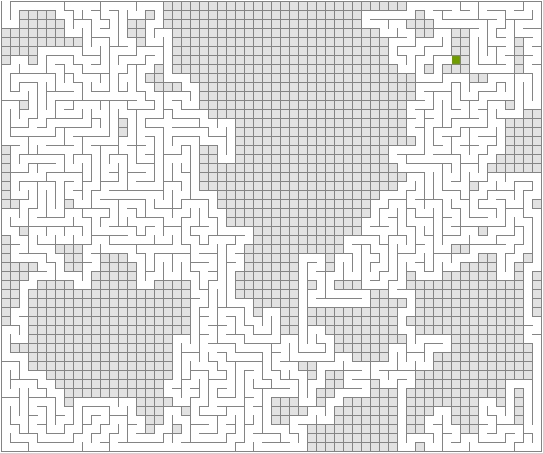
\includegraphics[scale=0.5]{MazeML-step-by-step-drawing.png}
  \end{figure}

  \vspace{3mm}
  \textbf{Remarque} : Cette fonctionnalité n'est pas disponible pour les 
  labyrinthes chargés à partir d'un fichier, car les informations de 
  backtracking nécessaires à l'animation sont perdues lors de l'enregistrement.


    \section{Historique des versions}

\noindent\textbf{Version 1.0} Première version proposée sur le SdZ.           \\
\textbf{Version 1.1} Optimisation selon les résultats du profiling (gprof).   \\
\textbf{Version 1.2} Simplification de la mise en mémoire de la solution.     \\
\textbf{Version 1.3} Meilleur affichage du chemin solution (tracé continu).   \\
\textbf{Version 1.4} Abandon des modifications de 1.3, nouvelle implémentation 
                     avec \texttt{Bigarray}                                   \\
\textbf{Version 1.5} Export au format PNG (avec transparence) ou JPEG.        \\
\textbf{Version 1.6} Tracé continu du chemin solution (restauration de 1.3).  \\
\textbf{Version 1.7} MazeML peut désormais construire pas à pas un labyrinthe.\\
\textbf{Version 1.8} Export de gros labyrinthes avec \texttt{--without-gui}.  \\
\textbf{Version 1.9} \emph{(à venir)} Version finale.

\end{document}
